
\section{HAR en Android}
\begin{frame}{HAR en Android}

\framesubtitle{Arquitectura del Proyecto}

\setbeamercovered{transparent}
\begin{columns}

\column{0.5\textwidth}
\begin{itemize}
\item \textbf{HARDroid} 
\begin{itemize}
\item Es un servicio utilitario de reconocimiento.
\item Clasificador din�mico
\end{itemize}

\pause{}
\item \textbf{ActivitySurvey}
\begin{itemize}
\item Aplicaci�n de encuesta que utiliza el servicio.
\item Registra las evaluaciones de los usuarios. 
\end{itemize}

\pause{}
\item \textbf{Backend C4.5} 
\begin{itemize}
\item Servicio web de recolecci�n de evaluaciones.
\item Aciertos utilizados para mejorar el clasificador.
\end{itemize}
\end{itemize}

\column{0.5\textwidth}
\begin{center}
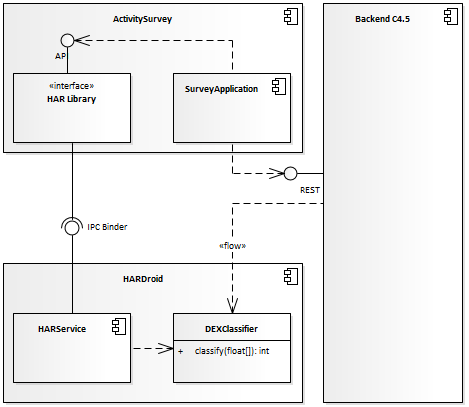
\includegraphics[width=1\columnwidth]{../capitulo-5/graphics/arqui_general}
\par\end{center}

\end{columns}

\end{frame}
%
\begin{frame}{HAR en Android}

\framesubtitle{Servicio de Reconocimiento}

\setbeamercovered{transparent}
\begin{columns}

\column{0.5\textwidth}
\begin{itemize}[<+->]
\item \structure{HARDroid} es un gestor en la capa de \emph{Application Framework}. 
\item Permite a aplicaciones m�viles hechas por terceros: 
\begin{itemize}
\item las �ltimas mejoras del motor de reconocimiento, 
\item actualizaci�n por plataforma de distribuci�n basado en tienda, 
\item los usuarios gozan actualizaciones r�pidas y los desarrolladores mecanismos
f�ciles de integraci�n.
\end{itemize}
\end{itemize}

\column{0.5\textwidth}
\begin{center}
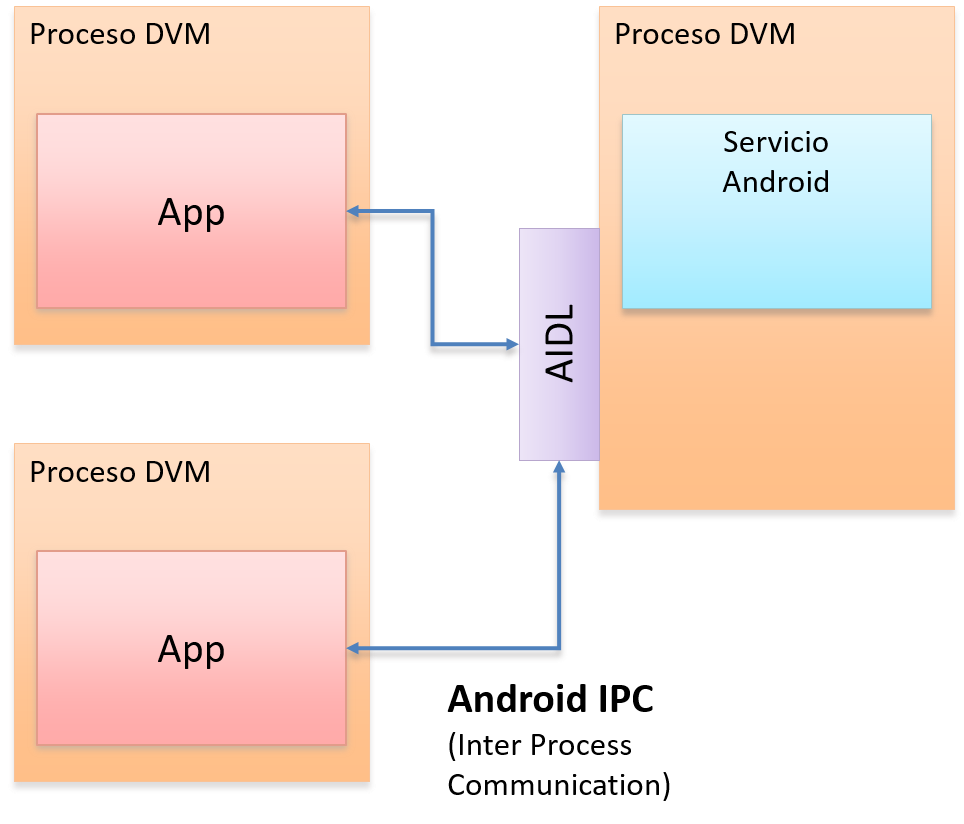
\includegraphics[width=1\columnwidth]{../capitulo-5/graphics/hardroid_func}
\par\end{center}

\end{columns}

\end{frame}
%
\begin{frame}{HAR en Android}

\framesubtitle{HARDroid: M�dulos Funcionales}
\begin{columns}[t]

\column{0.25\textwidth}
\begin{itemize}
\item Interfaz de Servicio 
\item Gestor
\item Procesador
\item Clasificador
\item Sensor
\end{itemize}

\column{0.75\textwidth}

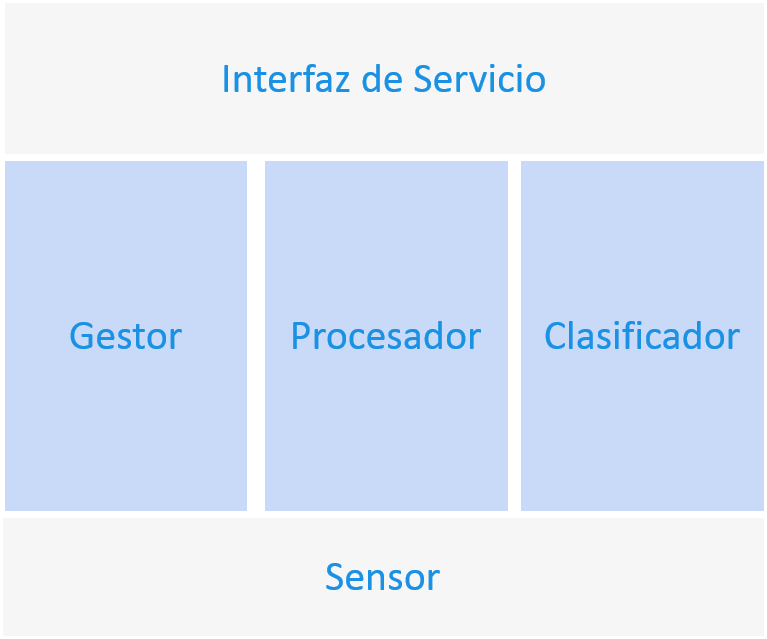
\includegraphics[width=1\columnwidth]{propuesta/graphics/hardroid}
\end{columns}

\end{frame}
%
\begin{frame}{HAR en Android}

\framesubtitle{Activity Survey: M�dulos Funcionales}
\begin{columns}[t]

\column{0.25\textwidth}
\begin{itemize}
\item Registro
\item Encuesta
\item Preferencias
\item Persistencia
\item Interfaz de Usuario
\end{itemize}

\column{0.75\textwidth}

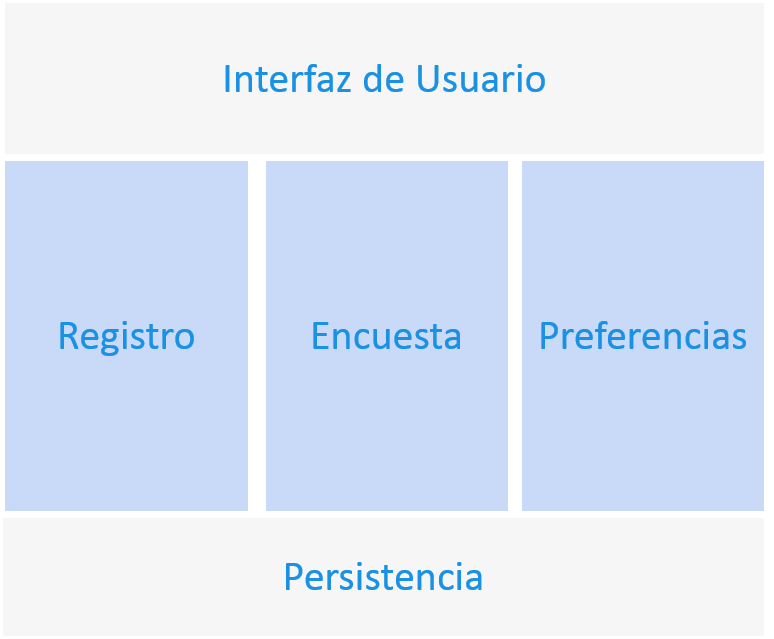
\includegraphics[width=1\columnwidth]{propuesta/graphics/activity_survey}
\end{columns}

\end{frame}
%
\begin{frame}{HAR en Android}


\framesubtitle{Activity Survey: Componentes Funcionales}
\begin{center}
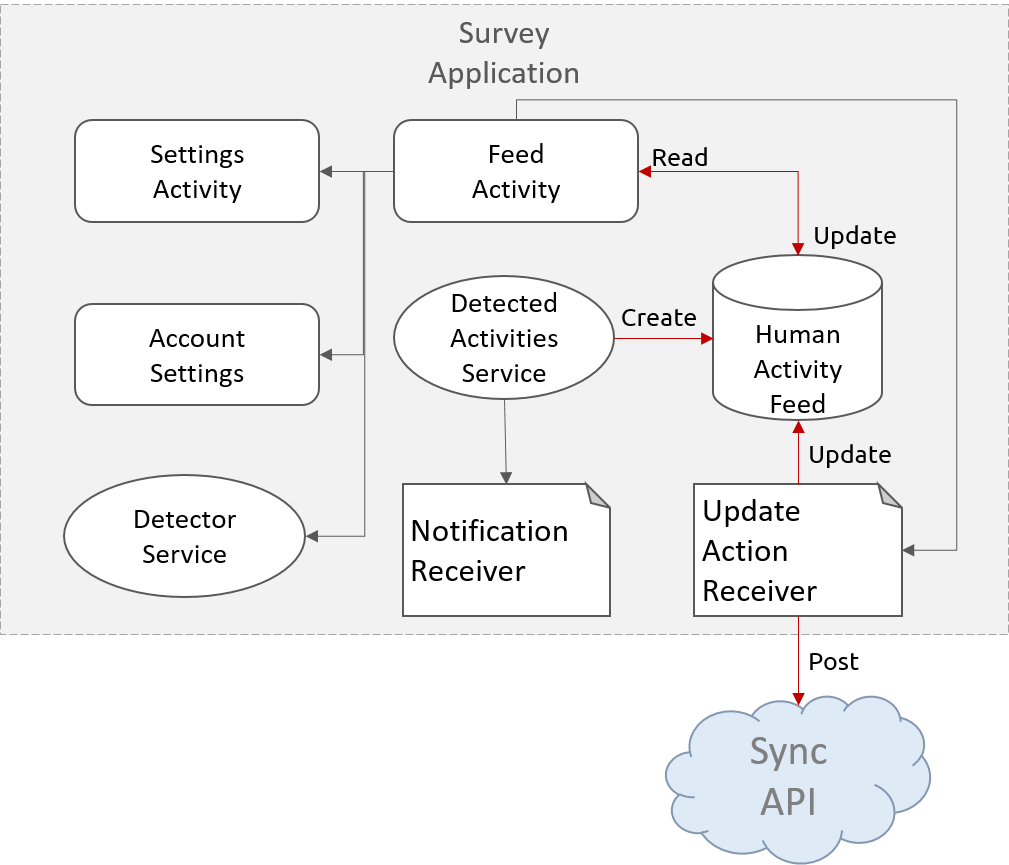
\includegraphics[width=0.65\columnwidth]{../capitulo-5/graphics/act_surv_diag}
\par\end{center}
\end{frame}

